% factor_graph.tex -- SLAM factor graph (tikz-bayesnet), GTSAM/Dellaert style.
% Variable nodes = circles (poses x_i, landmark l1); factor nodes = squares
% (prior, odometry, measurement). Factors placed at explicit midpoints (robust,
% no reliance on the 'between' key). Standalone; build via xelatex.
\documentclass[border=4pt]{standalone}
\usepackage{tikz}
\usetikzlibrary{bayesnet,calc}
\begin{document}
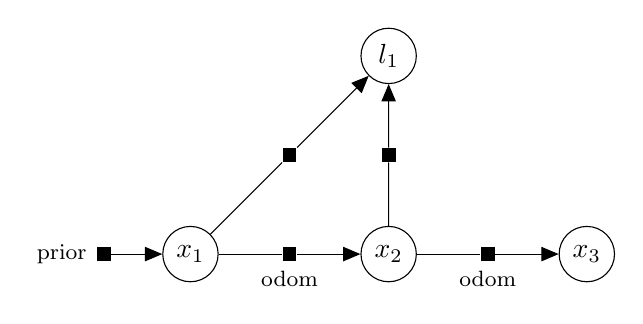
\begin{tikzpicture}
  % variable nodes (circles)
  \node[latent]                    (x1) {$x_1$};
  \node[latent, right=1.8cm of x1] (x2) {$x_2$};
  \node[latent, right=1.8cm of x2] (x3) {$x_3$};
  \node[latent, above=1.8cm of x2] (l1) {$l_1$};
  % factor nodes (small squares) at explicit midpoints
  \node[factor, label=left:prior]  (pri) at ($(x1)+(-1.1,0)$) {};
  \node[factor, label=below:odom]  (o1)  at ($(x1)!0.5!(x2)$) {};
  \node[factor, label=below:odom]  (o2)  at ($(x2)!0.5!(x3)$) {};
  \node[factor]                    (m1)  at ($(x1)!0.5!(l1)$) {};
  \node[factor]                    (m2)  at ($(x2)!0.5!(l1)$) {};
  % factor-edges (undirected) connecting each factor to its variables
  \factoredge {} {pri} {x1};
  \factoredge {x1} {o1} {x2};
  \factoredge {x2} {o2} {x3};
  \factoredge {x1} {m1} {l1};
  \factoredge {x2} {m2} {l1};
\end{tikzpicture}
\end{document}
